\documentclass{article}
\usepackage{graphicx} % Required for inserting images

\usepackage[french]{babel}
\usepackage[T1]{fontenc}
\usepackage{lmodern}
\usepackage{hyperref}
\usepackage{wrapfig}

\title{Rapport de projet : Chat201 – édition thread \& réseau}
\author{Daniel DEFOING (\texttt{ddef0003}) \and 
        Belinda ÖZNUR (\texttt{bozn0003}) \and
        Haluk YILMAZ (\texttt{hyil0003})}
\date{\today}

\begin{document}
\pagenumbering{gobble}

\maketitle
\tableofcontents
\newpage

\pagenumbering{arabic}
\section{Introduction}
Ce rapport décrit globalement la conception du second projet dans le cadre du cours de Systèmes d’Exploitation
(INFO-F201). Il présente les choix de conception qui ont guidé notre développement, et les difficultés qui ont pu survenir durant celui-ci. Pour voir de façon précise les changements ayant eu lieu tout au long du projet et la contribution de chacun, veuillez consulter \hyperref[https://github.com/Daniel-Dfg/OS_Projet_2]{le repository GitHub de notre projet}.

\section{Choix du langage :pourquoi C++ plutôt que C ?}

Une raison fondamentale qui a guidé cette décision est que C++ possède des fonctionnalités absentes
en C tels que les références, les chaînes de caractères (ou \textit{strings}) ou encore les classes. Or, dans le cadre du projet présenté ici, ces éléments apportent une pluvalue non négligeable :
\begin{itemize}
    \item Discuter des avantages du C++ (il y en a beaucoup)...
\end{itemize}
Ceci montre que des avantages majeurs ont été trouvés à utiliser C++ plutôt que C, alors qu’aucun avantage n’a été identifié en faveur de l’utilisation de C par rapport à C++. Ce choix du langage s’est donc naturellement imposé comme le plus adapté.

\section{Visualisation de l'architecture du programme}
Cette section discute des choix de conception du programme final, des considérations qui permettront au lecteur de mieux comprendre la nature de ces choix et des problèmes rencontrés qui en ont suivi.

\subsection{Le serveur en tant que point relais des clients}
La structure d'un programme client-serveur tel que celui présenté ici peut être visualisée très simplement sous la forme d'un Graphe Étoile \cite{Graphe Étoile}, avec le serveur au centre et les clients aux extrémités de chaque branche. 
\begin{figure}[ht]
    \centering
    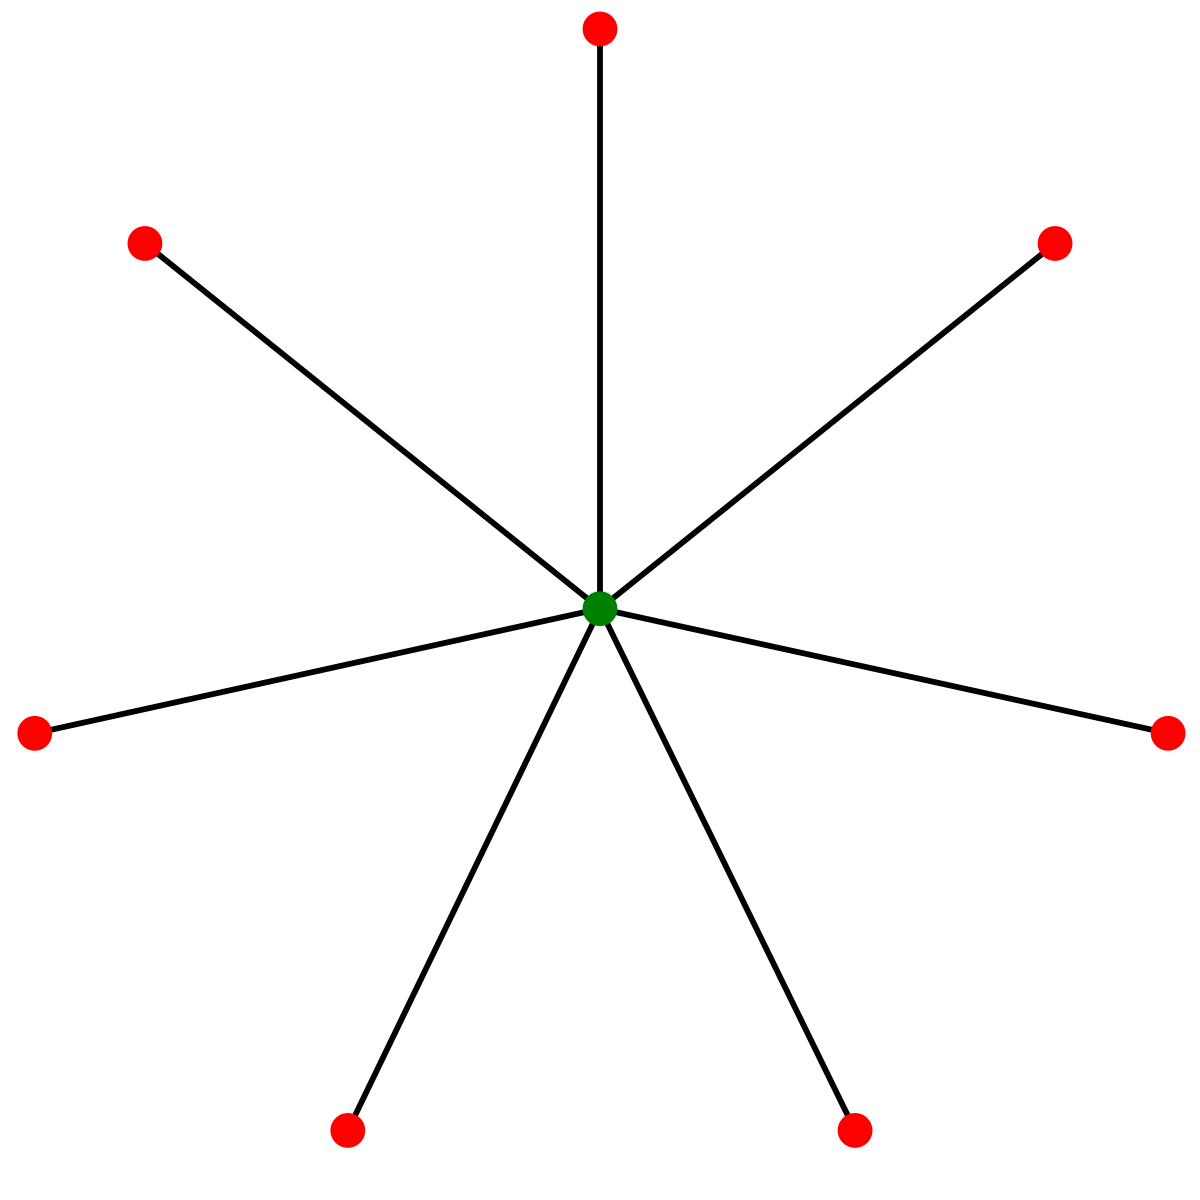
\includegraphics[width=0.25\linewidth]{etoile.png}
    \caption{\textit{Graphe Étoile typique.}}
\end{figure}

Cette représentation montre bien qu'un seul serveur se charge de \textit{relayer} les informations à passer d'un client à un autre ou d'un client vers lui-même (confirmation de (dé)connexion notamment). 

TODO : discuter du TCP/IP brièvement

Dans la suite, nous discuterons en profondeur de la façon dont les noeuds de ce graphe communiquent.

\subsection{Conceptions communes aux clients et au serveur}
\begin{itemize}
    \item 2 Queues à vider (par un nombre variables de threads selon qu'on est dans le client ou le serveur)
    \item Méthodes d'envoi des messages : utilisation d'une classe \texttt{Message}
    \item usage de \texttt{std::string} la plupart du temps
\end{itemize}

\subsection{Conception des clients}
\begin{itemize}
    \item 2 threads, 2 Queues (écho avec la section "Conceptions communes")
    \item Gestion de la connexion
    \item Gestion de la déconnexion (quel thread tue l'autre, comment on se déconnecte)
    \item ...
    
\end{itemize}

\subsection{Conception du serveur}
\begin{itemize}
    \item Plusieurs threads, 2 Queues (écho avec la section "Conceptions communes") : accès concurrents aux Queues, problème de producteur-consommateur
    \item Gestion des (dé)connexions
    \item Mapping des utilisateurs à leur file descriptors et inversement
    \item Gestion des sockets : surveillance permanente via \texttt{poll} (ou epoll le cas échéant)
    \item ...

\end{itemize}

\section{Difficultés rencontrées et solutions trouvées}
\subsection{Problèmes de synchronisation}
\begin{itemize}
    \item côté serveur, accès concurrents (problème producteur-consommateur)
    \item Signaux asynchrones (mentionner la conception du SignalManager dans l'explication de la solution)
    \item ...
\end{itemize}

\subsection{Garantie de l'intégrité du contenu partagé par les clients}
\begin{itemize}
    \item Gestion des tailles limites (longueur de pseudos et de messages)
    \item Comment s'est-on assurés que le messages étaient bien transmis sans perte ?
\end{itemize}


\begin{thebibliography}{999}
	\bibitem{Graphe Étoile}
		Wikipedia. (2019, 21 janvier). \textit{Graphe étoile.} URL: \url{https://fr.wikipedia.org/wiki/Graphe_%C3%A9toile}, consulté le 12/12/2024.
\end{thebibliography}
\end{document}

